\section{Datasets and Preprocessing}
\subsection{UCI Cleveland Heart Disease Dataset}
The Cleveland dataset (UCI repository, ID 45~\cite{janosi1989}) contains 303 patients referred for coronary angiography, each with 13 clinical variables (Table~\ref{tab:features}). The original target \texttt{num} (0--4) records angiographic disease status: 0 means $<$50\% diameter narrowing in every major vessel, and values 1--4 mean $>$50\% narrowing in at least one vessel~\cite{detrano1989}. Following common practice we binarise it as $y=1$ if \texttt{num}$>0$ (coronary artery disease, CAD) and $y=0$ otherwise. This gives \textbf{164 patients without CAD (54.1\%) and 139 with CAD (45.9\%)}. (The v4 manuscript paired these percentages with the wrong classes.) Table~\ref{tab:demo} summarises the cohort by class.

Two categorical variables have missing values: \texttt{ca} ($n=4$) and \texttt{thal} ($n=2$). Median imputation is used because the mean of a categorical code is not a valid category; rows are not dropped given the small cohort. \revnote{In this revision, the imputer, the feature derivation and the StandardScaler are fitted \emph{inside each training fold only} (Section~IV-G); in v4 they were fitted on all 303 patients before splitting.}

The variables \texttt{cp}, \texttt{restecg}, \texttt{slope} and \texttt{thal} are categorical codes. Standardising them as if they were continuous assumes equally spaced, ordered categories. This is harmless for tree models, which split on thresholds, but not for SVM or logistic regression. We therefore compare ordinal coding with one-hot coding in Section~VI-F.

\begin{table}[!t]
\centering\scriptsize
\caption{Cleveland Heart Disease dataset features.}
\label{tab:features}
\begin{adjustbox}{max width=\linewidth}
\begin{tabular}{lll}
\toprule
Feature & Description & Type\\
\midrule
age & Age in years & Continuous\\
sex & Sex (1 = male, 0 = female) & Binary\\
cp & Chest-pain type (1--4; 4 = asymptomatic) & Categorical\\
trestbps & Resting blood pressure (mm Hg) & Continuous\\
chol & Serum cholesterol (mg/dL) & Continuous\\
fbs & Fasting blood sugar $>$ 120 mg/dL & Binary\\
restecg & Resting ECG (0 normal, 1 ST-T abnormality, 2 LVH) & Categorical\\
thalach & Maximum heart rate achieved & Continuous\\
exang & Exercise-induced angina & Binary\\
oldpeak & ST depression, exercise vs.\ rest & Continuous\\
slope & Peak-exercise ST slope (1 up, 2 flat, 3 down) & Ordinal\\
ca & Major vessels coloured by fluoroscopy (0--3) & Ordinal\\
thal & Thallium scan (3 normal, 6 fixed, 7 reversible defect) & Categorical\\
\bottomrule
\end{tabular}
\end{adjustbox}
\end{table}

\begin{table}[!t]
\centering
\scriptsize
\caption{Cleveland cohort by class (mean $\pm$ SD or n (\%); Mann--Whitney U or $\chi^2$ test).}
\label{tab:demo}
\setlength{\tabcolsep}{3pt}
\begin{adjustbox}{max width=\linewidth}
\begin{tabular}{lccc}
\toprule
Characteristic & No CAD & CAD & $p$ \\
\midrule
Patients, n & 164 & 139 & -- \\
Age, years & 52.6 $\pm$ 9.5 & 56.6 $\pm$ 7.9 & $<$0.001 \\
Female, n (\%) & 72 (44\%) & 25 (18\%) & $<$0.001 \\
Asymptomatic chest pain & 39 (24\%) & 105 (76\%) & $<$0.001 \\
Resting BP, mm Hg & 129.2 $\pm$ 16.2 & 134.6 $\pm$ 18.8 & 0.026 \\
Cholesterol, mg/dL & 242.6 $\pm$ 53.5 & 251.5 $\pm$ 49.5 & 0.035 \\
Max.\ heart rate & 158.4 $\pm$ 19.2 & 139.3 $\pm$ 22.6 & $<$0.001 \\
Exercise angina & 23 (14\%) & 76 (55\%) & $<$0.001 \\
ST depression (oldpeak) & 0.6 $\pm$ 0.8 & 1.6 $\pm$ 1.3 & $<$0.001 \\
Fasting glucose $>$120 & 23 (14\%) & 22 (16\%) & 0.781 \\
\bottomrule
\end{tabular}
\end{adjustbox}
\end{table}


\subsection{Additional UCI Sites for External Validation}
The same repository holds patients from three further centres with identical variable definitions: the Hungarian Institute of Cardiology, Budapest ($n=294$); University Hospitals Zurich and Basel ($n=123$); and the VA Medical Center, Long Beach ($n=200$). They were not used for training. We use them only as external test sets (Section~VI-G). Their disease prevalence differs from Cleveland and many tests are missing (Table~\ref{tab:sites}). Cholesterol recorded as 0~mg/dL is physiologically impossible and is treated as missing.

\subsection{PTB-XL ECG Dataset}
PTB-XL~\cite{wagner2020} provides ten-second 12-lead ECGs sampled at 500~Hz (100~Hz version also available), tagged with SCP-ECG diagnostic statements. We use version 1.0.3 from PhysioNet~\cite{wagner2022ptbxl103} (21{,}799 records from 18{,}869 patients after removal of duplicates; the Kaggle copy used for v4 listed 21{,}837 records). A record is labelled normal ($y=0$) only when \texttt{NORM} is its sole diagnostic statement with non-zero likelihood, and abnormal ($y=1$) otherwise, giving 9{,}097 normal and 12{,}702 abnormal records. A proportionally stratified sample of 303 records (126 normal, 177 abnormal; seed 42) matches the Cleveland cohort size.

\textbf{Label semantics.} PTB-XL labels are broad \emph{ECG diagnostic categories} (myocardial infarction, conduction disturbance, ST/T change, hypertrophy and so on), not angiographic coronary narrowing. A PTB-XL ``abnormal'' label and a Cleveland ``CAD'' label are therefore different constructs, and ECG-only scores on PTB-XL cannot be compared directly with Cleveland scores.

\textbf{Single-lead choice.} Feature extraction uses Lead~II, which lies close to the mean electrical axis, shows P waves and QRS morphology clearly, and is the standard rhythm-strip lead~\cite{kligfield2007}. A single lead, however, loses spatial information: ischaemia and infarction are localised by the territory of the leads that show them (e.g.\ V1--V4 anterior, II/III/aVF inferior), and vector-cardiographic features such as the QRS axis need several leads. We accept this limitation to keep the tsfresh feature space manageable for $N=303$, and we quantify it by comparing Leads I, II, V1 and V5 and a 12-lead representation (Section~VI-J). Fig.~\ref{fig:ptbxl} gives an overview of the sample.

\begin{figure}[!t]
\centering
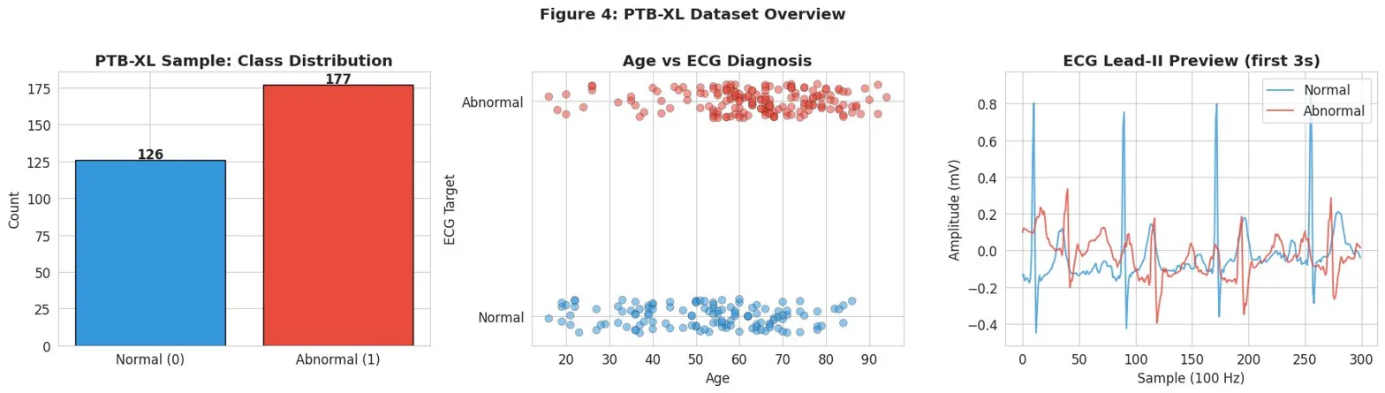
\includegraphics[width=\linewidth]{fig1_ptbxl_overview.png}
\caption{PTB-XL sample: class distribution, age versus diagnosis, and Lead-II traces (first 3~s).}
\label{fig:ptbxl}
\end{figure}

\subsection{ECG Feature Extraction}
Each Lead-II signal (1{,}000 samples at 100~Hz) is converted to the long format expected by tsfresh~\cite{christ2018} and processed with \texttt{EfficientFCParameters}, which yields 777 descriptors: time-domain statistics, autocorrelation, trend, entropy, spectral (FFT, Welch) and non-linear measures (c3, CID-CE, time-reversal asymmetry). tsfresh is suitable for fixed-length 10-s segments because its features are computed over the whole window and do not require beat segmentation~\cite{christ2018}. A VarianceThreshold filter ($\tau=0.01$) leaves 568 descriptors (in v4 this filter was fitted on all records; in this revision it is fitted inside each training fold).

\subsection{Datasets Used in This Study}
Table~\ref{tab:mapping} maps each dataset to its rows, features, label and the models trained on it (reviewer request).

\begin{table}[!t]
\centering\scriptsize
\caption{Dataset-to-model mapping.}
\label{tab:mapping}
\setlength{\tabcolsep}{2pt}
\begin{adjustbox}{max width=\linewidth}
\begin{tabular}{>{\raggedright\arraybackslash}p{1.15cm}>{\raggedright\arraybackslash}p{1.0cm}>{\raggedright\arraybackslash}p{1.35cm}>{\raggedright\arraybackslash}p{1.2cm}>{\raggedright\arraybackslash}p{2.55cm}}
\toprule
Dataset & Rows & Features & Label & Used for / models\\
\midrule
D1 Cleveland & 303 & 13 clinical & CAD (num$>$0) & Clinical-only baseline; LR, SVM, RF, XGB, GBM, voting, MLP\\
D3 Cleveland & 303 & 13 clinical + 23 ECG-proxy & CAD & Proposed system; all ablations (Sec.~VI-A--I)\\
D2 PTB-XL & 303 (1,212) & 568 tsfresh (Lead II) & ECG normal vs.\ abnormal & Parallel ECG benchmark (Sec.~VI-J); not fused with D1/D3\\
External & 294, 123, 200 & as D1/D3 & CAD & Test only (Sec.~VI-G)\\
\bottomrule
\end{tabular}
\end{adjustbox}
\end{table}
